\chapter{ทฤษฎีการตัดสินใจ (Decision Theory)}

\section*{โจทย์ธุรกิจ}
\begin{tcolorbox}[colback=white!100!white, colframe=black!80!white,
  title=ข้อความ,
  fonttitle=\bfseries,
  sharp corners=southwest,
  boxrule=0.8pt,
  left=1mm, right=1mm, top=1mm, bottom=1mm,
]
\emph{
``ขอบคุณสำหรับแผนการผลิตที่คุณแนะนำครับ แต่เรายังมีปัญหาใหม่เกิดขึ้น...  
ฝ่ายบริหารกำลังลังเลว่าจะใช้กลยุทธ์ไหนต่อในไตรมาสหน้า  
เพราะสถานการณ์ตลาดมีแนวโน้มเปลี่ยนแปลงตลอดเวลา  
บางสัปดาห์โต๊ะทำงานขายดี บางสัปดาห์กลับเป็นตู้เอกสารที่มาแรง  
บางทีก็มีปัญหาขนส่งวัตถุดิบจากซัพพลายเออร์อีก  
ถ้าจะวางกลยุทธ์ที่เหมาะสม เราควรเลือกแนวทางการผลิตแบบใด?"}
\end{tcolorbox}
คุณสมชายกลับมาอีกครั้ง หลังจากบริษัท ABC Furniture ใช้แบบจำลองเชิงเส้นเพื่อตัดสินใจจำนวนการผลิตโต๊ะทำงานและตู้เก็บเอกสารในแต่ละสัปดาห์ได้แล้ว ซึ่งทำให้ได้ผลดีในช่วงแรก ๆ ที่ใช้งาน แต่ผ่านไปสักพักฝ่ายการตลาดพบว่ามีปัจจัยภายนอกมากระทบทำให้ไม่สามารถใช้แค่เกณฑ์ภายในด้านกำไรมาพิจารณาได้อย่างเดียว และสถานการณ์ตลาดเปลี่ยนแปลงอย่างรวดเร็ว — ทำให้ฝ่ายการผลิตต้องเผชิญกับความไม่แน่นอนหลายด้าน เช่น
\begin{itemize}
    \item ราคาขายเปลี่ยนแปลง
    \item ความต้องการของลูกค้าเปลี่ยนไป
    \item มีปัญหาการขนส่งวัตถุดิบ
    \item คู่แข่งออกรุ่นใหม่ที่มีราคาถูกกว่า
\end{itemize}~
เพื่อช่วยในการวางแผน บริษัทจึงอยากรู้ว่า หากมีสถานการณ์ที่ไม่แน่นอน (uncertain states of nature) เกิดขึ้น บริษัทควรเลือกแนวทางการผลิตแบบใดเพื่อรับมือ

\textbf{คำถามชวนคิด:}
\begin{itemize}
    \item คุณคิดว่าบริษัท ABC Furniture กำลังเผชิญกับปัญหาแบบใด? ทำไม LP ไม่ตอบโจทย์?
    \item คุณต้องการข้อมูลอะไรเพิ่มเติมก่อนจะตอบคำถามของคุณสมชายได้?
    \item คุณจะเริ่มต้นจัดกลุ่มหรือจำแนกทางเลือกในการตัดสินใจอย่างไร?
    \item หากไม่สามารถรู้อนาคตได้แน่ชัด คุณจะวิเคราะห์หรือวางแผนอย่างไร?
    \item ลองจินตนาการว่าบริษัทอาจมี “หลายสถานการณ์ตลาด” ที่อาจเกิดขึ้น คุณจะจัดโครงสร้างปัญหาเพื่อเปรียบเทียบตัวเลือกได้อย่างไร?
    \item คุณคาดหวังว่าข้อมูลลักษณะใดจะช่วยให้การตัดสินใจแม่นยำมากขึ้น?
\end{itemize}

\section*{บทนำ}
(Draft Version)\footnote{draft for teaching in class, not for text book this semester}

\begin{itemize}
    \item ในบางครั้ง ก็มีทางเลือกที่จะต้องตัดสินใจเลือก
    \item เป้าหมายคือทางเลือกที่ดีที่สุด
    \item แต่ก็มีรูปแบบของสถานการณ์ได้หลากหลาย ขึ้นกับการเกิดขึ้นของทางเลือกที่มี: (1) ภายใต้ความแน่นอน (2) ภายใต้ความเสี่ยง และ (3) ภายใต้ความไม่แน่นอน
    \item ซึ่งการตัดสินใจภายใต้ความเสี่ยงและความไม่แน่นอนนั้นจะใช้ทฤษฎีความน่าจะเป็นเข้ามาช่วย: ค่าคาดหวัง (expected value)
\end{itemize}

\section{ลักษณะการแสดงข้อมูล}
เราสามารถแสดงข้อมูลเพื่อความง่ายในการอ่านได้ 2 รูปดังนี้
\begin{enumerate}
    \item เมทริกซ์การตัดสินใจ (decision matrix) เป็นการแสดงผลจากลัพธ์ (เช่น กำไร) ระหว่างตัวเลือก (option) และเหตุการณ์ที่เป็นไปได้ที่อาจจะเกิดขึ้น
    \begin{center}
        \begin{tabular}{c|c|c|c|c|}
             & เหตุการณ์ 1 & เหตุการณ์ 2 & $\cdots$ & เหตุการณ์ $n$ \\ \hline
            ทางเลือก 1 &  & & & \\
            ทางเลือก 2 &  & & & \\
            $\vdots$ &  & & & \\
            ทางเลือก $m$ &  & & & \\ \hline
        \end{tabular}
    \end{center}
        
    \item ต้นไม้การตัดสินใจ (decision tree) เป็นลักษณะของการแสดงความต่อเนื่องของเหตุการณ์การเลือกโดยอาศัยจุดยอด (node) เชื่อมต่อกัน และปลายกิ่งสุดท้ายจะแสดงผลลัพธ์ที่เกิดขึ้น
    \begin{figure}[h!]
        \centering
        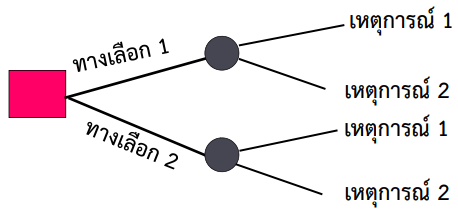
\includegraphics[width=0.5\linewidth]{decisiontree.png}
        \caption{Enter Caption}
        \label{fig:enter-label}
    \end{figure}
\end{enumerate}

\begin{example}
    {ตัวอย่างการสร้างเมทริกซ์การตัดสินใจ และต้นไม้การตัดสินใจ}{decision-matrix}
    ณ บริษัทสมมติแห่งหนึ่ง ต้องการตัดสินใจว่าจะจัดนิทรรศการขนาดเล็ก หรือขนาดกลาง หรือขนาดใหญ่ โดยจากการประเมิณเบื้องต้นพบว่าถ้าขายบัตรเข้างานได้หมด จะได้กำไร 8 ล้านบาท, 15 ล้านบาท และ 25 ล้านบาทเรียงตามขนาดของงาน ในขณะที่ถ้าขายได้ 50\% ของบัตรทั้งหมดจะได้กำไร 4 ล้านบาท, 15 ล้านบาท และ 10 ล้านบาทตามลำดับ และถ้าขายได้เพียงแค่ 10\% ของบัตรทั้งหมดจะได้กำไร 3 บาท และขาดทุน 1 ล้านบาทและ 10 ล้านบาทตามลำดับขนาดของงาน จากเหตุการณ์ดังกล่าว จะสร้างเมทริกซ์การตัดสินใจและต้นไม้การตัดสินใจได้ดังนี้
\end{example}
\newpage

\section{การตัดสินใจภายใต้สภาวะความแน่นอน}
\begin{itemize}
    \item เมื่อทราบว่าจะเกิดเหตุการณ์ใดขึ้น
    \item ถึงจะไม่ realistic ในหลาย ๆ กรณี แต่บางครั้งเราก็ต้องพิจารณาในรูปแบบนี้
    \item เพราะง่ายและตรงไปตรงมา
\end{itemize}

\begin{example}
    {การตัดสินใจภายใต้สภาวะความแน่นอน}{}
    จากเมทริกซ์การตัดสินใจที่ได้จากตัวอย่าง \ref{ex:decision-matrix} จะตัดสินใจภายใต้สภาวะความแน่นอนของแต่ละเหตุการณ์ได้อย่างไรบ้าง
\end{example}

\newpage
\section{การตัดสินใจภายใต้สภาวะความเสี่ยง}
\begin{itemize}
    \item ไม่ทราบว่าจะเกิดเหตุการณ์ใด
    \item แต่พอมีข้อมูลเพื่อคาดการณ์ความน่าจะเป็นของการเกิดแต่ละเหตุการณ์ได้
    \item ใช้แนวคิดเรื่องของความน่าจะเป็นเข้ามาช่วย
\end{itemize}
\subsection{ค่าคาดหวัง (Expected Value)}
\begin{definition}
    {ค่าคาดหวัง}{}
    ภายใต้การทดลองเชิงการสุ่มหนึ่ง ถ้าผลจอบแทนทั้งหมดที่เป็นไปได้คือ $X = X_1, X_2, X_3, \dots$ (อาจจะมีจำกัดหรือไม่จำกัดเหตุการณ์ก็ได้) โดยที่มีความน่าจะเป็นการได้ผลตอบแทนเป็น $P(X) = P(X_1), P(X_2), P(X_3), \dots$ ตามลำดับ
    แล้ว\textbf{ค่าคาดหวัง}ของผลตอบแทนจะคำนวณโดย
    $$
    E(X) := X_1 P(X_1) + X_2 P(X_2) + X_3 P(X_3) + \cdots
    $$
\end{definition}
ซึ่งค่าคาดหวังในเชิงความน่าจะเป็นเปรียบเสมือนค่าเฉลี่ยในเชิงสถิติที่จะบอกแนวโน้มการได้ว่ามักจะได้ค่าไหนเป็นส่วนใหญ่
\begin{example}
    {ค่าคาดหวังของเหตุการณ์อย่างง่าย}{}
    สมมติว่าพนันด้วยการโยนเหรียญไม่เที่ยงตรงอันหนึ่งโดยมีโอกาสออกหัว 0.3 และออกก้อย 0.7 ในการพนันนี้มีกฏว่าถ้าออกหัวผู้เล่นจะได้เงิน 5 บาท ในขณะที่ถ้าออกก้อยผู้เล่นจะเสียเงิน 3 บาท ในการเล่นพนันครั้งนี้ผู้เล่นจะเสียเปรียบหรือว่าได้เปรียบอยู่กี่บาท
\end{example}

\newpage
\subsection{เกณฑ์ผลตอบแทน}
\begin{example}
    {การตัดสินใจภายใต้สภาวะความเสี่ยง:ค่าคาดหวังของผลตอบแทน}{}
    จากเมทริกซ์การตัดสินใจที่ได้จากตัวอย่าง \ref{ex:decision-matrix} ซึ่งคือ
    \begin{center}
        \begin{tabular}{|c|c|c|c|}
        \hline
            (หน่วย: ล้านบาท) & ขายได้หมด & ขายได้ 50\% & ขายได้ 10\% \\ \hline
            ขนาดเล็ก & 8 & 4 & 3 \\
            ขนาดกลาง & 15 & 15 & -1\\
            ขนาดใหญ่ & 25 & 10 & -10\\ \hline
        \end{tabular}
    \end{center}
    และจากการสำรวจสถิติเก่า ๆ พบว่า โอกาสที่จะขายได้หมดมี 0.3 ในขณะที่ขายได้ครึ่งหนึ่งของงานจะมีโอกาสที่ 0.4 และขายได้เพียง 10\% ของงานจะมีโอกาสอยู่ที่ 0.3
    เนื่องจากเราไม่ทราบว่าจะเกิดเหตุการณ์แบบไหนขึ้น แต่เราทราบความน่าจะเป็นที่จะเกิด เราจึงต้องใช้ค่าคาดหวังเข้ามาช่วย 
    \begin{enumerate}
        \item เราต้องหาค่าคาดหวังของอะไร (ระบุตัวแปรสุ่ม) โดยที่แยกคิดตามอะไร (ตามขนาดงานหรือตามปริมาณการขายบัตรได้)
        \item จงหาค่าคาดหวังตามที่ตั้งไว้
        \item และจากค่าคาดหวังที่ได้ ควรเลือกจัดงานขนาดใด
        \item ข้อมูลเรื่องความน่าจะเป็นที่จะเกิดเหตุการณ์ต่าง ๆ นักศึกษาคิดว่าหาได้จากไหนบ้าง (ยกตัวอย่างแหล่งข้อมูล หรือสิ่งที่ขอเพิ่มจากลูกค้า)
    \end{enumerate}
\end{example}
\newpage
\subsection{เกณฑ์ค่าเสียโอกาส (opportunity loss)}
\begin{itemize}
    \item นอกจากคำนวณจากผลตอบแทนแล้ว เรายังสามารถคำนวณโดยอาศัยเกณฑ์ค่าเสียโอกาส
    \item ค่าเสียโอกาส = ผลตอบแทนที่ควรได้สูงสุด - ผลตอบแทนกรณีเลือกตัวเลือกดังกล่าว
    \item และใช้ค่าคาดหวังของค่าเสียโอกาส (Expected Opportunity Loss: EOL) เป็นตัวตัดสินใจ
\end{itemize}
\begin{example}
    {การตัดสินใจภายใต้สภาวะความเสี่ยง:ค่าคาดหวังของค่าเสียโอกาส}{}
    จากเมทริกซ์การตัดสินใจที่ได้จากตัวอย่าง \ref{ex:decision-matrix} ซึ่งคือ
    \begin{center}
        \begin{tabular}{|c|c|c|c|}
        \hline
            (หน่วย: ล้านบาท) & ขายได้หมด & ขายได้ 50\% & ขายได้ 10\% \\ \hline
            ขนาดเล็ก & 8 & 4 & 3 \\
            ขนาดกลาง & 15 & 15 & -1\\
            ขนาดใหญ่ & 25 & 10 & -10\\ \hline
        \end{tabular}
    \end{center}
    และจากการสำรวจสถิติเก่า ๆ พบว่า โอกาสที่จะขายได้หมดมี 0.3 ในขณะที่ขายได้ครึ่งหนึ่งของงานจะมีโอกาสที่ 0.4 และขายได้เพียง 10\% ของงานจะมีโอกาสอยู่ที่ 0.3
    เนื่องจากเราไม่ทราบว่าจะเกิดเหตุการณ์แบบไหนขึ้น แต่เราทราบความน่าจะเป็นที่จะเกิด เราจึงต้องใช้ค่าคาดหวังเข้ามาช่วย 
    \begin{enumerate}
        \item จงคำนวณค่าเสียโอกาสที่จะเกิดขึ้นในแต่ละเหตุการณ์
        \item จงหาค่าคาดหวังของค่าเสียโอกาส
        \item และจากค่าคาดหวังที่ได้ ควรเลือกจัดงานขนาดใด
    \end{enumerate}
\end{example}
\newpage
\subsection{ค่าคาดหวังของข่าวสารที่สมบูรณ์}
\begin{itemize}
    \item ถ้าเราทราบเหตุการณ์ที่จะเกิดได้ จะทำให้เลือกตัวเลือกที่ทำกำไรได้สูงสุดแน่นอน (มีข่าวสารสมบูรณ์)
    $$
    \text{ค่าคาดหวังของข่าวสารที่สมบูรณ์} = E(\text{ผลตอบแทนสูงสุดของแต่ละเหตุการณ์})
    $$
    \item แต่ถ้าเราไม่มีข่าวสารอะไรเลย เราจะตัดสินใจได้เพียงแค่ค่าคาดหวังของผลตอบแทนในแต่ละตัวเลือก และเลือกตัวเลือกที่ให้ค่าคาดหวังมากที่สุด
    $$
    \text{ค่าคาดหวังที่สูงที่สุดเมื่อไม่มีข่าวสาร} = \max_\text{ตัวเลือก}E(\text{ผลตอบแทนตามเหตุการณ์})
    $$
    \item เราจึงวัดผลความต่างระหว่างค่าคาดหวังที่จะทำผลตอบแทนได้สูงสุดเมื่อมีข่าวสารสมบูรณ์เทียบกับค่าคาดหวังที่สูงที่สุดเมื่อไม่มีข่าวสาร
    \item เรียกว่า \textbf{ค่าคาดหวังของข่าวสารที่สมบูรณ์} (Expected Value of Perfect Information: EVPI)
    $$
    EVPI = \text{ค่าคาดหวังเมื่อมีข่าวสารสมบูรณ์} - \text{ค่าคาดหวังที่สูงที่สุดเมื่อไม่มีข่าวสาร}
    $$
\end{itemize}
\begin{example}
    {การตัดสินใจภายใต้สภาวะความเสี่ยง:ค่าคาดหวังของข่าวสารที่สมบูรณ์}{}
    จากเมทริกซ์การตัดสินใจที่ได้จากตัวอย่าง \ref{ex:decision-matrix} ซึ่งคือ
    \begin{center}
        \begin{tabular}{|c|c|c|c|}
        \hline
            (หน่วย: ล้านบาท) & ขายได้หมด & ขายได้ 50\% & ขายได้ 10\% \\ \hline
            ขนาดเล็ก & 8 & 4 & 3 \\
            ขนาดกลาง & 15 & 15 & -1\\
            ขนาดใหญ่ & 25 & 10 & -10\\ \hline
        \end{tabular}
    \end{center}
    และจากการสำรวจสถิติเก่า ๆ พบว่า โอกาสที่จะขายได้หมดมี 0.3 ในขณะที่ขายได้ครึ่งหนึ่งของงานจะมีโอกาสที่ 0.4 และขายได้เพียง 10\% ของงานจะมีโอกาสอยู่ที่ 0.3 จงคำนวณหา EVPI และอภิปรายค่าที่ได้ในแง่ของการลงทุนทำ R\&D เพิ่มเติม 
\end{example}
\newpage
ผลพลอยได้อย่างหนึ่งที่น่าสนใจคือไม่ว่าเราจะใช้เกณฑ์ใดก็ตาม เราจะได้วิธีการตัดสินใจเดียวกันเสมอ
\begin{theorem}
    {ปัญหาคู่กันของเกณฑ์ผลตอบแทนและเกณฑ์ค่าเสียโอกาส}{mon-eol}
    ผลการตัดสินใจที่ได้จากค่าคาดหวังของผลตอบแทนจะเหมือนกับผลการตัดสินใจจากค่าคาดหวังของค่าเสียโอกาส
    $$
    \arg\max_{\text{ตัวเลือก}} E(\text{ผลตอบแทน}) = \arg\min_{\text{ตัวเลือก}} E(\text{ค่าเสียโอกาส})
    $$
\end{theorem}
และทำให้เราได้ผลตามมาว่า
\begin{corollary}
    {EVPI กับ EOL}{}
    $$
    EVPI = \min_{\text{ตัวเลือก}} E(\text{ค่าเสียโอกาส})
    $$
\end{corollary}
(ข้ามได้) เพื่อความง่ายสำหรับนักศึกษาที่ไม่คุ้นเคยกับการคิดคณิตศาสตร์แบบนามธรรม ขอกำหนดให้เรามีทางเลือก 3 ทางเลือก และเหตุการณ์ 4 เหตุการณ์ 
% (แต่ถ้านักศึกษาชอบความท้าทาย อาจจะลองคิดแบบใด ๆ คือ $m$ ทางเลือกและ $n$ เหตุการณ์เลยก็ได้)
    \begin{exercise}
        {คำถามช่วยไกด์}{}
        \begin{enumerate}
            \item กำหนดให้เมทริกซ์ผลตอบแทนคือ $D=\begin{bmatrix}
                                                x_{11} & x_{12} & x_{13} & x_{14} \\
                                                x_{21} & x_{22} & x_{23} & x_{24} \\
                                                x_{31} & x_{32} & x_{33} & x_{34}
                                                \end{bmatrix}$ และเวกเตอร์ความน่าจะเป็นคือ $\vec{p} = \begin{bmatrix}
                                                p_{1}\\
                                                p_{2}\\
                                                p_{3}\\
                                                p_{4}
                                                \end{bmatrix}$ แล้วเราจะสามารถใช้ $D$ และ $\vec{p}$ เขียนแสดงค่าคาดหวังของผลตอบแทนได้อย่างไร\\(Ans: $\vec{E}(\text{ผลตอบแทน}) = D\vec{p}$)
            \item เพื่อที่จะเขียนเมทริกซ์ที่แสดงถึงค่าเสียโอกาส ขอสมมติว่าให้ในเหตุการณ์ที่ 1, 2, 3 และ 4 มีผลตอบแทนที่ได้มากที่สุดเป็น $x_{11}, x_{32}, x_{23}, x_{24}$ ตามลำดับ กล่าวคือในเหตุการณ์ที่ 1, 2, 3 และ 4 นั้นทางเลือกที่ 1, 3, 2 และ 2 จะให้ผลตอบแทนเยอะสุดตามลำดับ จงเขียนค่าเสียโอกาสรายตัวเลือกให้อยู่ในรูปเมทริกซ์
            \item ถ้าไม่กำหนดแบบเจาะจงว่าตัวเลือกใดให้ผลตอบแทนมากที่สุดในแต่ละเหตุการณ์ แต่สมมติว่าให้ผลตอบแทนที่มากที่สุดของเหตุการณ์ที่ 1, 2, 3 และ 4 มีผลตอบแทนที่ได้มากที่สุดเป็น $M_1, M_2, M_3, M_4$ ตามลำดับ จงเขียนค่าเสียโอกาสรายตัวเลือกให้อยู่ในรูปเมทริกซ์\\(Ans: $M - D$ โดยที่ทุกแถวของ $M$ คือ $M_1, M_2, M_3, M_4$)
            \item จงหาค่าคาดหวังของค่าเสียโอกาส\\(Ans: $\vec{E}(\text{ค่าเสียโอกาส}) = M\vec{p} - D\vec{p}$)
            \item คราวนี้เราจะสามารถพิสูจน์ผลใน \ref{thm:mon-eol} โดยใช้ผลจากข้อ 1 และข้อ 4
        \end{enumerate}
    \end{exercise}
    
\section{การตัดสินใจภายใต้สภาวะที่ไม่แน่นอน}
% ในหลายๆ สถานการณ์นั้น เรามักไม่ทราบโอกาสการเกิดของแต่ละเหตุการณ์เลย ไม่เหมือนกรณีภายใต้ความเสี่ยงที่เรายังสามารถประมาณการณ์การเกิดได้ด้วยความน่าจะเป็น ดังนั้นเราจึงทำได้เพียงแค่การใช้เกณฑ์การเปรียบเทียบเชิงมากกว่าน้อยกว่าได้เท่านั้น

\begin{tcolorbox}[colback=white!100!white, colframe=black!80!white,
  title=maximax criterion,
  fonttitle=\bfseries,
  sharp corners=southwest,
  boxrule=0.8pt,
  left=1mm, right=1mm, top=1mm, bottom=1mm,
]
เหมาะกับผู้ตัดสินใจที่มีนิสัยกล้าได้กล้าเสีย โดยเลือกค่าผลลัพธ์สูงสุด (Maximum payoff) ของแต่ละทางเลือก แล้วเลือกค่าที่มากที่สุดในบรรดานั้น

\[
\text{Maximax} = \max_i \left( \max_j \, a_{ij} \right)
\]

โดยที่ $a_{ij}$ คือค่าผลลัพธ์ของกลยุทธ์ $i$ เมื่อเกิดเหตุการณ์ $j$
\end{tcolorbox}

\begin{tcolorbox}[colback=white!100!white, colframe=black!80!white,
  title=maximin criterion,
  fonttitle=\bfseries,
  sharp corners=southwest,
  boxrule=0.8pt,
  left=1mm, right=1mm, top=1mm, bottom=1mm,
]
เหมาะกับผู้ตัดสินใจที่ระมัดระวัง โดยเลือกค่าผลลัพธ์ต่ำสุด (Minimum payoff) ของแต่ละทางเลือก แล้วเลือกค่าที่มากที่สุดในบรรดานั้น

\[
\text{Maximin} = \max_i \left( \min_j \, a_{ij} \right)
\]
\end{tcolorbox}

\begin{tcolorbox}[colback=white!100!white, colframe=black!80!white,
  title=minimax regret criterion,
  fonttitle=\bfseries,
  sharp corners=southwest,
  boxrule=0.8pt,
  left=1mm, right=1mm, top=1mm, bottom=1mm,
]
คำนวณ “ความเสียใจ” (regret) โดยการหาผลต่างระหว่างผลลัพธ์ที่ดีที่สุดในแต่ละสถานการณ์ กับค่าของแต่ละกลยุทธ์ แล้วเลือกกลยุทธ์ที่มี regret สูงสุดน้อยที่สุด

\[
r_{ij} = \max_i a_{ij} - a_{ij}, \quad
\text{Minimax Regret} = \min_i \left( \max_j \, r_{ij} \right)
\]
\end{tcolorbox}

\begin{tcolorbox}[colback=white!100!white, colframe=black!80!white,
  title=Laplace criterion,
  fonttitle=\bfseries,
  sharp corners=southwest,
  boxrule=0.8pt,
  left=1mm, right=1mm, top=1mm, bottom=1mm,
]
ถือว่าทุกสถานการณ์มีโอกาสเกิดเท่ากัน แล้วคำนวณค่าเฉลี่ยของแต่ละกลยุทธ์ จากนั้นเลือกค่าที่มีค่าเฉลี่ยสูงสุด

\[
\text{Laplace} = \max_i \left( \frac{1}{n} \sum_{j=1}^n a_{ij} \right)
\]

โดยที่ $n$ คือจำนวนเหตุการณ์ที่เป็นไปได้
\end{tcolorbox}

\begin{tcolorbox}[colback=white!100!white, colframe=black!80!white,
  title=Hurwicz criterion,
  fonttitle=\bfseries,
  sharp corners=southwest,
  boxrule=0.8pt,
  left=1mm, right=1mm, top=1mm, bottom=1mm,
]
ประนีประนอมระหว่าง maximax และ maximin โดยใช้ค่าสัมประสิทธิ์ $\alpha$ ที่สะท้อนระดับความมองโลกในแง่ดี

\[
\text{Hurwicz}_i = \alpha \cdot \max_j a_{ij} + (1 - \alpha) \cdot \min_j a_{ij}
\]

โดย $0 \leq \alpha \leq 1$ และเลือกกลยุทธ์ที่ให้ค่าดังกล่าวสูงสุด
\end{tcolorbox}

\begin{example}
    {การตัดสินใจภายใต้สภาวะความไม่แน่นอน}{}
    จากเมทริกซ์การตัดสินใจที่ได้จากตัวอย่าง \ref{ex:decision-matrix} ซึ่งคือ
    \begin{center}
        \begin{tabular}{|c|c|c|c|}
        \hline
            (หน่วย: ล้านบาท) & ขายได้หมด & ขายได้ 50\% & ขายได้ 10\% \\ \hline
            ขนาดเล็ก & 8 & 4 & 3 \\
            ขนาดกลาง & 15 & 15 & -1\\
            ขนาดใหญ่ & 25 & 10 & -10\\ \hline
        \end{tabular}
    \end{center}
    จงคำนวณค่าตามเกณฑ์ต่าง ๆ และเปรียบเทียบผลการตัดสินใจที่ได้ 
\end{example}
\newpage
\section{การใช้ต้นไม้การตัดสินใจ}
ไม่ใช่การคำนวณใหม่ แต่เป็นวิธีการคิดสิ่งเดิมโดยใช้แผนภาพเข้ามาช่วย
\subsection{การคิดค่าคาดหวังด้วยแผนภาพต้นไม้ความน่าจะเป็นของเหตุการณ์}
การคิดเกี่ยวกับเหตุการณ์ความน่าจะเป็นนั้นสามารถเขียนในรูปแบบการวาดแผนภาพต้นไม้เพื่อพิจารณาเหตุการณ์ที่เกิดขึ้นต่อเนื่องกัน ตัวอย่างเช่น การโยนเหรียญ 2 เหรียญต่อเนื่องกัน โดยเหรียญแรกเป็นเหรียญไม่เที่ยงตรงที่มีโอกาสออกหัว 0.7 และออกก้อย 0.3 ในขณะที่เหรียญที่สองเป็นเหรียญที่มีโอกาสออกหัว 0.4 และออกก้อย 0.6 ถ้าเราพิจารณาความน่าจะเป็นที่จะได้ เราสามรถวาดแผนภาพได้ดังนี้
\begin{center}
\begin{tikzpicture}[>=Stealth, node distance=2cm and 2cm, font=\sffamily]

% จุดเริ่มต้น
\node (start) [circle, fill=black!20, minimum size=10pt] {};

% เหรียญแรก: H (0.7), T (0.3)
\node[right=of start, yshift=1.5cm] (H1) [circle, fill=gray!50] {H};
\node[right=of start, yshift=-1.5cm] (T1) [circle, fill=gray!50] {T};

% เหรียญสองจาก H1: H (0.4), T (0.6)
\node[right=of H1, yshift=1cm] (HH) {HH};
\node[right=of H1, yshift=-1cm] (HT) {HT};

% เหรียญสองจาก T1: H (0.4), T (0.6)
\node[right=of T1, yshift=1cm] (TH) {TH};
\node[right=of T1, yshift=-1cm] (TT) {TT};

% เส้นเหรียญ 1
\draw[->] (start) -- (H1) node[midway, above left] {H (0.7)};
\draw[->] (start) -- (T1) node[midway, below left] {T (0.3)};

% เส้นเหรียญ 2 (จาก H1)
\draw[->] (H1) -- (HH) node[midway, above] {H (0.4)};
\draw[->] (H1) -- (HT) node[midway, below] {T (0.6)};

% เส้นเหรียญ 2 (จาก T1)
\draw[->] (T1) -- (TH) node[midway, above] {H (0.4)};
\draw[->] (T1) -- (TT) node[midway, below] {T (0.6)};

\end{tikzpicture}
\end{center}
ซึ่งสามารถนำมาช่วยคิดค่าความน่าจะเป็นได้โดยอาศัยลักษณะการคูณของสายต่อเนื่อง เช่น\footnote{เราพิจารณากรณีง่าย ซึ่งคือกรณีที่เหตุการณ์ทั้ง 2 ขั้นตอนอิสระจากกัน}
$$
P(HT) = P(H)P(T) = 0.7 \times 0.6 = 0.42
$$

และในกรณีที่มีเรื่องของผลลัพท์เพื่อนำมาคิดค่าคาดหวังของผลลัพธ์นั้น เราอาจจะเขียนแผนภาพต้นไม้เพิ่มเติมได้ดังนี้
\begin{center}
\begin{tikzpicture}[>=Stealth, node distance=2cm and 2cm, font=\sffamily]

% จุดเริ่มต้น
\node (start) [circle, fill=black!20, minimum size=10pt] {};

% เหรียญแรก: H (0.7), T (0.3)
\node[right=of start, yshift=1.5cm] (H1) [circle, fill=gray!50] {H};
\node[right=of start, yshift=-1.5cm] (T1) [circle, fill=gray!50] {T};

% เหรียญสองจาก H1: H (0.4), T (0.6)
\node[right=of H1, yshift=1cm] (HH) {HH: -500 บาท};
\node[right=of H1, yshift=-1cm] (HT) {HT: 300 บาท};

% เหรียญสองจาก T1: H (0.4), T (0.6)
\node[right=of T1, yshift=1cm] (TH) {TH: 400 บาท};
\node[right=of T1, yshift=-1cm] (TT) {TT: -500 บาท};

% เส้นเหรียญ 1
\draw[->] (start) -- (H1) node[midway, above left] {H (0.7)};
\draw[->] (start) -- (T1) node[midway, below left] {T (0.3)};

% เส้นเหรียญ 2 (จาก H1)
\draw[->] (H1) -- (HH) node[midway, above] {H (0.4)};
\draw[->] (H1) -- (HT) node[midway, below] {T (0.6)};

% เส้นเหรียญ 2 (จาก T1)
\draw[->] (T1) -- (TH) node[midway, above] {H (0.4)};
\draw[->] (T1) -- (TT) node[midway, below] {T (0.6)};

\end{tikzpicture}
\end{center}
ซึ่งเราสามารถคิดค่าคาดหวังของผลลัพธ์ได้ตามแบบนิยามของค่าคาดหวังได้เป็น 
\begin{align*}
    E(\text{ผลลัพธ์}) &= -500P(HH) + 300P(HT) + 400P(TH) - 500P(TT)\\
                    &= -500(0.7)(0.4) + 300(0.7)(0.6) + 400(0.3)(0.4) - 500(0.3)(0.6)
\end{align*}

แต่ถ้าพิจารณาตามลำดับขั้นการคำนวณตามแผนภาพต้นไม้ เราสามารถจัดรูปได้เป็น
\begin{align*}
    E(\text{ผลลัพธ์}) &= -500(0.7)(0.4) + 300(0.7)(0.6) + 400(0.3)(0.4) - 500(0.3)(0.6)\\
                    &= (-500(0.4) + 300(0.6))(0.7)+ (400(0.4) - 500(0.6))(0.3)\\
                    &= \text{ค่าคาดหวังที่ต้นไม่ย่อยที่เหรียญแรกออกหัว}(0.7) + \text{ค่าคาดหวังที่ต้นไม่ย่อยที่เหรียญแรกออกก้อย}(0.3)
\end{align*}
\begin{center}
\begin{tikzpicture}[>=Stealth, node distance=2cm and 2cm, font=\sffamily]

% จุดเริ่มต้น
\node (start) [circle, fill=black!20, minimum size=10pt] {};

% เหรียญแรก: H (0.7), T (0.3)
\node[right=of start, yshift=1.5cm] (H1) [circle, fill=gray!50] {H};
\node[right=of H1, xshift=-2cm] {: $-500(0.4) + 300(0.6)$};
\node[right=of start, yshift=-1.5cm] (T1) [circle, fill=gray!50] {T};
\node[right=of T1, xshift=-2cm] {: $400(0.4) - 500(0.6)$};

% เส้นเหรียญ 1
\draw[->] (start) -- (H1) node[midway, above left] {H (0.7)};
\draw[->] (start) -- (T1) node[midway, below left] {T (0.3)};

\node[below=of start, yshift=-1.5cm] (start_new) [circle, fill=black!20, minimum size=10pt] {};
\node[right=of start_new, xshift=-1cm] {: $(-500(0.4) + 300(0.6))(0.7)+ (400(0.4) - 500(0.6))(0.3)$};
\end{tikzpicture}
\end{center}

กล่าวคือ ในกรณีที่เรามีแผนภาพลำดับของการเกิดเหตุกาเมื่รณ์ในรูปแบบของแผนภาพต้นไม้ เราสามารถคิดค่าคาดหวังของทั้งต้นไม้นั้นได้โดยคิดจาดค่าคาดหวังของต้นไม้ย่อยก่อน หรือก็คือคิดไต่ขึ้นมาจากปลายกิ่งไล่ไปหาจุดรากของแผนภาพ

\subsection{เมื่อมีตัวเลือกเข้ามาเกี่ยวข้อง}
ความแตกต่างสำคัญระหว่างตัวเลือกและเหตุการณ์คือ ตัวเลือกเป็นสิ่งที่เรากำหนดให้เป็นขึ้นกับข้อมูลที่มี ในขณะที่เหตุการณ์คือสิ่งที่เราควบคุมไม่ได้ ยิ่งเฉพาะในการตัดสินใจภายใต้ความเสี่ยงนั้น เหตุการณ์จะเป็นสิ่งที่มีค่าความน่าจะเป็นมาเป็นตัวควบคุมโอกาสที่จะเกิด

ในหัวข้อที่ผ่านมา เป็นพื้นฐานการคำนวณค่าความน่าจะเป็นและค่าคาดหวังโดยใข้แผนภาพต้นไม้เป็นเครื่องมือช่วยให้เราคำนวยณได้อย่างเป็นระบบมากขึ้น ซึ่งมีเพียงแค่ลำดับของเหตุการณ์ที่เข้ามาพิจารณาเท่านั้น ยังไม่มีตัวเลือกอยู่ในแผนภาพต้นไม้

เมื่อมีตัวเลือกเข้ามาเกี่ยวข้อง แผนภาพต้นไม้จะไม่สามารถคิดด้วยหลักความน่าจะเป็นของทั้งแผนภาพได้ แต่จะใช้วิธีการตัดสินใจเลือกตัวเลือกไล่ลำดับไปจากปลายกิ่งไปราก (ขวาไปซ้าย) โดยการเลือกทางเลือกที่ให้ค่าคาดหวังของผลตอบแทนที่มากที่สุด

\begin{example}
    {การตัดสินใจโดยใช้ต้นไม้การตัดสินใจ}{}
    จากเหตุการณ์ในตัวอย่าง \ref{ex:decision-matrix} เราจะสามารถวาดแผนภาพต้นไม้ได้ดังนี้
    \begin{center}
        \begin{tikzpicture}[>=Stealth, node distance=2.8cm and 2.5cm, font=\sffamily]
        
        % สี่เหลี่ยม ตัดสินใจ
        \node[draw, rectangle, fill=orange!50, minimum width=0.2cm, minimum height=1cm] (dec) {};
        % \node (D) {decision};
        
        % นิทรรศการ 3 ทางเลือก
        \node[draw, circle, fill=gray!30, right=of dec, yshift=2.5cm] (S) {เล็ก};
        \node[draw, circle, fill=gray!30, right=of dec] (M) {กลาง};
        \node[draw, circle, fill=gray!30, right=of dec, yshift=-2.5cm] (L) {ใหญ่};
        
        % เหตุการณ์จากทางเลือก "เล็ก"
        \node[right=of S, yshift=0.75cm] (S1) {(all: 0.3) profit = 8M};
        \node[right=of S] (S2) {(half: 0.4) profit = 4M};
        \node[right=of S, yshift=-0.75cm] (S3) {(few: 0.3) profit = 3M};
        
        % % จาก "กลาง"
        \node[right=of M, yshift=0.75cm] (M1) {(all: 0.3) profit = 15M};
        \node[right=of M] (M2) {(half: 0.4) profit = 15M};
        \node[right=of M, yshift=-0.75cm] (M3) {(few: 0.3) profit = -1M};
        
        % % จาก "ใหญ่"
        \node[right=of L, yshift=0.75cm] (L1) {(all: 0.3) profit = 25M};
        \node[right=of L] (L2) {(half: 0.4) profit = 10M};
        \node[right=of L, yshift=-0.75cm] (L3) {(few: 0.3) profit = -10M};
        
        % เส้นจากตัดสินใจไปทางเลือก
        \draw[->] (dec) -- (S) node[midway, above left] {small};
        \draw[->] (dec) -- (M) node[midway, above] {medium};
        \draw[->] (dec) -- (L) node[midway, below left] {large};
        
        % % เส้นผลลัพธ์แต่ละทาง
        \draw[->] (S) -- (S1);
        \draw[->] (S) -- (S2);
        \draw[->] (S) -- (S3);
        \draw[->] (M) -- (M1);
        \draw[->] (M) -- (M2);
        \draw[->] (M) -- (M3);
        \draw[->] (L) -- (L1);
        \draw[->] (L) -- (L2);
        \draw[->] (L) -- (L3);
        \end{tikzpicture}
    \end{center}
    โดยที่โอกาสที่จะขายได้หมดมี 0.3 ในขณะที่ขายได้ครึ่งหนึ่งของงานจะมีโอกาสที่ 0.4 และขายได้เพียง 10\% ของงานจะมีโอกาสอยู่ที่ 0.3 
    จงเขียนขั้นตอนการตัดสินใจโดยใช้แผนภาพต้นไม้การตัดสินนี้ (แบ่งส่วนแผนภาพต้นไม้ความน่าจะเป็นขึ้นมาก่อนเพื่อหาค่าคาดหวัง แล้วค่อยตัดสินใจด้วยค่าคาดหวังของแต่ละต้นไม้ย่อย)
\end{example}
\newpage
\begin{example}
    {การตัดสินใจโดยใช้ต้นไม้การตัดสินใจ 2}{}
    บริษัท ABC กำลังพิจารณาว่าควรจะเปิดตัวผลิตภัณฑ์ใหม่เข้าสู่ตลาดหรือไม่ โดยมีทางเลือกหลายขั้นตอนซับซ้อนที่ต้องประเมินต้นทุน ความไม่แน่นอน และผลตอบแทนที่อาจเกิดขึ้น ดังนี้:

\begin{itemize}
    \item \textbf{ขั้นตอนที่ 1: การทดสอบผลิตภัณฑ์}
    \begin{itemize}
        \item บริษัทสามารถเลือกที่จะทำการทดสอบผลิตภัณฑ์ก่อน โดยมีโอกาส:
        \begin{itemize}
            \item \(80\%\) ที่ผลิตภัณฑ์ \textbf{ผ่าน} การทดสอบ
            \item \(20\%\) ที่ผลิตภัณฑ์ \textbf{ไม่ผ่าน} การทดสอบ และบริษัทจะขาดทุนทันที 100,000 บาท
        \end{itemize}
        \item หากผ่านการทดสอบ จะเข้าสู่ขั้นตอนถัดไป คือการทดสอบตลาด
    \end{itemize}

    \item \textbf{ขั้นตอนที่ 2: การทดสอบตลาด}
    \begin{itemize}
        \item ผลิตภัณฑ์ที่ผ่านการทดสอบ จะถูกนำไปทดสอบตลาดกับกลุ่มลูกค้าตัวอย่าง โดยมีโอกาส:
        \begin{itemize}
            \item \(90\%\) ที่ตลาด \textbf{ยอมรับผลิตภัณฑ์ใหม่}
            \item \(10\%\) ที่ตลาด \textbf{ไม่ยอมรับ} และบริษัทจะขาดทุน 250,000 บาท
        \end{itemize}
        \item หากตลาดยอมรับ จะเข้าสู่การตัดสินใจว่าจะนำผลิตภัณฑ์เข้าสู่ตลาดหรือไม่
    \end{itemize}

    \item \textbf{ขั้นตอนที่ 3: การตัดสินใจเปิดตัวผลิตภัณฑ์ }
    \begin{enumerate}
        \item \textbf{หากเปิดตัวผลิตภัณฑ์} ความสำเร็จในตลาดมีระดับและผลตอบแทนต่างกัน:
        \begin{itemize}
            \item ยอดขายสูง (\(40\%\)) $\rightarrow$ กำไร 1,450,000 บาท
            \item ยอดขายปานกลาง (\(40\%\)) $\rightarrow$ กำไร 450,000 บาท
            \item ยอดขายต่ำ (\(20\%\)) $\rightarrow$ ขาดทุน 150,000 บาท
        \end{itemize}
        \item \textbf{หากไม่เปิดตัว} จะยอมขาดทุนค่าทดสอบตลาด 250,000 บาท
    \end{enumerate}

    \item \textbf{ทางเลือกทางลัด: ข้ามการทดสอบผลิตภัณฑ์และเข้าสู่ตลาดทันที}
    \begin{itemize}
        \item หากบริษัทเลือกข้ามขั้นตอนและนำผลิตภัณฑ์เข้าสู่ตลาดทันที:
        \begin{itemize}
            \item ยอดขายสูง (\(10\%\)) $\rightarrow$ กำไร 1,700,000 บาท
            \item ยอดขายปานกลาง (\(40\%\)) $\rightarrow$ กำไร 700,000 บาท
            \item ยอดขายต่ำ (\(50\%\)) $\rightarrow$ กำไร 100,000 บาท
        \end{itemize}
    \end{itemize}
\end{itemize}

\medskip
\noindent
บริษัทควรดำเนินการตามทางเลือกใด เพื่อให้ได้ \textbf{ผลตอบแทนคาดหวังสูงสุด} ภายใต้ต้นทุนและความไม่แน่นอนในแต่ละขั้นตอน?

  
\end{example}
\newpage~
% 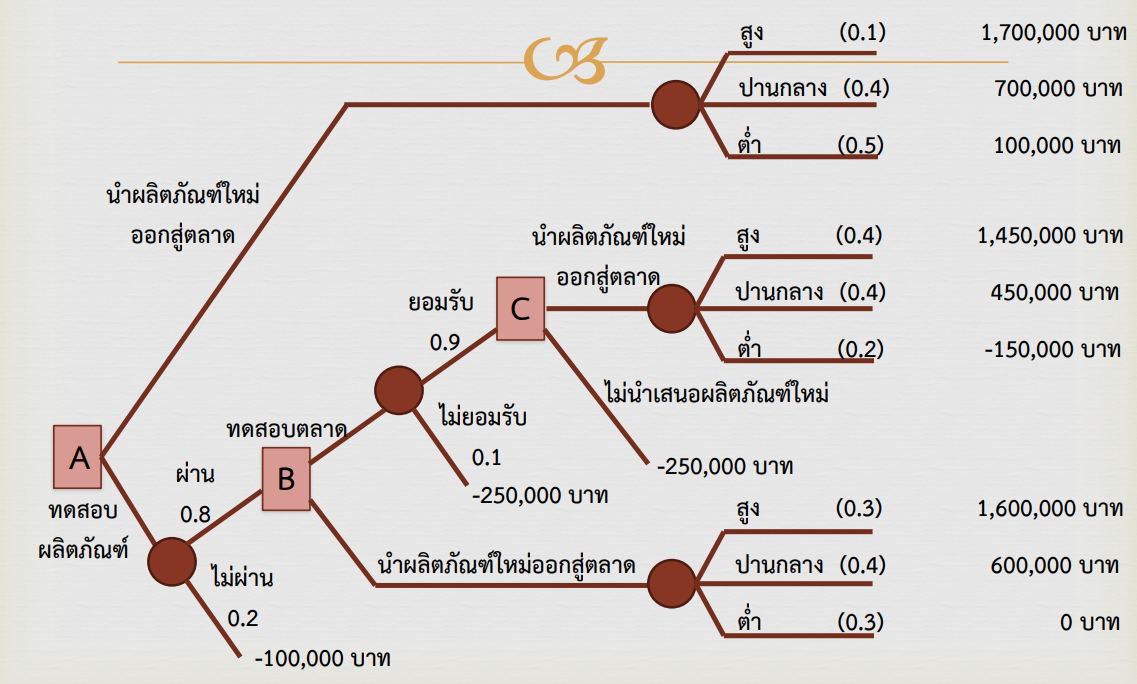
\includegraphics[width=1\linewidth]{solx.png}
\newpage
\section{การใช้โปรแกรม QM for Windows}
\newpage
\section*{Assignment (need revise)}
\subsection*{PART A:}
หลังจากบริษัท ABC Furniture ได้ใช้การวิเคราะห์เชิงเส้นในการวางแผนการผลิตช่วงไตรมาสก่อนหน้า  
บริษัทได้รับผลลัพธ์ที่ดีในช่วงแรก แต่ปัจจุบันกลับพบว่าไม่สามารถพึ่งพาแบบจำลองเดิมได้ตลอดเวลา  
เนื่องจากมีความไม่แน่นอนในตลาดสูงขึ้นเรื่อย ๆ เช่น ราคาวัตถุดิบผันผวน การแข่งขันสูง และความต้องการของลูกค้าที่แปรเปลี่ยนตลอด

\medskip
\noindent
\textbf{สถานการณ์ทางเลือก:} สำหรับไตรมาสถัดไป ฝ่ายผลิตเสนอ 3 กลยุทธ์ให้ฝ่ายบริหารพิจารณา:

\begin{itemize}
    \item \textbf{กลยุทธ์ A:} เพิ่มกำลังผลิต “โต๊ะทำงาน” ให้มากที่สุด โดยลดสัดส่วนตู้เก็บเอกสารลง
    \item \textbf{กลยุทธ์ B:} เพิ่มกำลังผลิต “ตู้เก็บเอกสาร” ให้มากที่สุด โดยลดสัดส่วนโต๊ะทำงานลง
    \item \textbf{กลยุทธ์ C:} กระจายการผลิตแบบสมดุลระหว่างทั้งสองประเภท
\end{itemize}

\noindent
\textbf{สถานการณ์ตลาด (States of Nature):}  
ฝ่ายการตลาดระบุว่าสถานการณ์ตลาดอาจเป็นไปได้ 3 แบบในไตรมาสหน้า:

\begin{itemize}
    \item \textbf{สถานการณ์ 1 (S1) — โต๊ะบูม:} โต๊ะทำงานขายดีมาก ตู้ขายได้น้อย
    \item \textbf{สถานการณ์ 2 (S2) — ตลาดสมดุล:} สินค้าทั้งสองขายได้ใกล้เคียงกัน
    \item \textbf{สถานการณ์ 3 (S3) — ตู้บูม:} ตู้เอกสารขายดีมาก โต๊ะขายได้น้อย
\end{itemize}

ฝ่ายบริหารต้องการทราบว่า ภายใต้แต่ละกลยุทธ์นั้น ถ้าเกิดสถานการณ์ตลาดแต่ละแบบ จะได้กำไรเท่าไร โดยฝ่ายวิเคราะห์ประเมินกำไร (หน่วย: พันบาท) ดังตาราง:

\begin{center}
\begin{tabular}{|c|c|c|c|}
\hline
\textbf{กลยุทธ์การผลิต} & \textbf{S1: โต๊ะบูม} & \textbf{S2: สมดุล} & \textbf{S3: ตู้บูม} \\
\hline
A (เน้นโต๊ะ) & 1,500 & 900 & 100 \\
B (เน้นตู้) & 200 & 800 & 1,400 \\
C (สมดุล) & 800 & 850 & 700 \\
\hline
\end{tabular}
\end{center}

\vspace{1em}
\noindent
\textbf{คำสั่ง:}

\begin{enumerate}
    % \item เขียนตารางผลตอบแทน (Payoff Table) จากข้อมูลข้างต้น (หากยังไม่ได้)
    \item วิเคราะห์การตัดสินใจภายใต้ความไม่แน่นอน โดยใช้เกณฑ์ต่อไปนี้:
    \begin{itemize}
        \item Maximax Criterion
        \item Maximin Criterion
        \item Laplace Criterion
        \item Hurwicz Criterion (ใช้ $\alpha = 0.6$)
        \item Minimax Regret Criterion
    \end{itemize}
    \item แต่ละเกณฑ์แนะนำกลยุทธ์ใด? อธิบายว่าแต่ละเกณฑ์สะท้อนทัศนคติความเสี่ยงแบบใด?
    \item ใช้โปรแกรม \textbf{QM for Windows} เพื่อคำนวณและตรวจสอบผลลัพธ์ พร้อมแนบภาพประกอบผลลัพธ์
\end{enumerate}

\subsection*{PART B:}
หลังจากฝ่ายบริหารบริษัท ABC Furniture ได้พิจารณาตารางผลตอบแทนจากกลยุทธ์ต่าง ๆ แล้ว  
ยังคงมีความลังเล เนื่องจากบริษัทไม่สามารถคาดการณ์สถานการณ์ตลาดล่วงหน้าได้อย่างแม่นยำ

คุณสมชายจึงเสนอแนวคิดว่า \emph{“หากบริษัทจ้างนักวิเคราะห์ตลาดมืออาชีพมาช่วยประเมินแนวโน้มตลาดก่อนได้หรือไม่?”}  
ซึ่งจะมีค่าใช้จ่ายในการจ้างทีมวิเคราะห์ภายนอกอยู่ที่ 150,000 บาท  
ทีมวิเคราะห์จะให้ผลลัพธ์เป็น \textbf{สัญญาณตลาดล่วงหน้า} (Market Signal) ซึ่งแบ่งเป็น 2 แบบคือ:

\begin{itemize}
    \item \textbf{สัญญาณบวก (Positive Signal):} แสดงว่าตลาดมีแนวโน้มดี
    \item \textbf{สัญญาณลบ (Negative Signal):} แสดงว่าตลาดมีแนวโน้มผันผวนหรือถดถอย
\end{itemize}

บริษัทสามารถเลือกที่จะ “เปิดกลยุทธ์ A, B หรือ C” หลังจากได้รับสัญญาณจากนักวิเคราะห์ก็ได้  
หรือจะตัดสินใจ “ไม่เปลี่ยนแผน” ก็ได้เช่นกัน

\medskip
\noindent
\textbf{ข้อมูลความแม่นยำของนักวิเคราะห์ตลาด} จากประวัติ:
\begin{itemize}
    \item หากสถานการณ์ตลาดเป็น \textbf{S1 (โต๊ะบูม)} $\rightarrow$ ให้สัญญาณบวก 80\%, สัญญาณลบ 20\%
    \item หากสถานการณ์ตลาดเป็น \textbf{S2 (สมดุล)} $\rightarrow$ ให้สัญญาณบวก 50\%, สัญญาณลบ 50\%
    \item หากสถานการณ์ตลาดเป็น \textbf{S3 (ตู้บูม)} $\rightarrow$ ให้สัญญาณบวก 30\%, สัญญาณลบ 70\%
\end{itemize}

\noindent
\textbf{ความน่าจะเป็นของแต่ละสถานการณ์ตลาด} (ตามฝ่ายการตลาดประเมิน):  
S1: 25\%, S2: 50\%, S3: 25\%

\medskip
\noindent
\textbf{คำสั่ง:}

\begin{enumerate}
    \item วาดแผนภาพ Decision Tree ที่เริ่มจากทางเลือก “จ้างนักวิเคราะห์” หรือ “ไม่จ้าง”
    \item แสดงการแตกเหตุการณ์ตามลำดับ: สัญญาณ → สถานการณ์ตลาด → กลยุทธ์การผลิต → ผลตอบแทนสุทธิ (หักค่าจ้าง)
    \item คำนวณ \textbf{Expected Monetary Value (EMV)} ของแต่ละทางเลือก (รวมต้นทุน 150,000 กรณีที่จ้าง)
    \item สร้างโมเดลนี้ใน \textbf{QM for Windows} เพื่อยืนยันผลลัพธ์ พร้อมแนบภาพผลลัพธ์
    \item คุณคิดว่าการจ้างนักวิเคราะห์มีความคุ้มค่าหรือไม่?
\end{enumerate}